\documentclass[presentation]{beamer}
\usepackage[utf8]{inputenc}
\usepackage[T1]{fontenc}
\usepackage[ngerman]{babel}
\usepackage{graphicx}
\usepackage{textcomp}
\usepackage{marvosym}
\usetheme{Szeged}
\usecolortheme{seagull}
\setbeamertemplate{blocks}[rectangles]
\hypersetup{colorlinks=true, urlcolor=blue}

\title{Grundlagen zu (verteilten) Versionskontrollsystemen}
\author[Michael Markert]{Michael Markert\\
  \href{mailto:markert.michael@googlemail.com}{markert.michael@googlemail.com}\\
  \url{https://github.com/cofi}}
\date{\today}

\AtBeginSection[]
{
  \begin{frame}<beamer>
    \tableofcontents[currentsection]
  \end{frame}
}

\begin{document}
\begin{frame}[plain]
  \titlepage
\end{frame}

\begin{frame}{Outline}
  \setcounter{tocdepth}{1}
  \tableofcontents
\end{frame}
\section{Versionskontrolle}
\begin{frame}{Definitionen}
  \begin{definition}<1->
    Ein \alert{Changeset} ist eine atomare Gruppe \textbf{zusammenhängender}
    Veränderungen und wird durch einen \textbf{Commit} erzeugt.
  \end{definition}
  \begin{definition}<2->
    Ein \alert{Repository} ist der Ort in dem ein Versionskontrollsystem seine
    Daten ablegt.
  \end{definition}
\end{frame}
\begin{frame}{Definitionen II}
  \begin{definition}<1->
    Ein \alert{zentralisiertes Versionskontrollsystem} besitzt genau ein
    gemeinsam benutztes Repository. Benutzer arbeiten auf einem
    \emph{Snapshot}(Checkout).
  \end{definition}
  \begin{definition}<2->
    Ein \alert{dezentralisiertes Versionskontrollsystem} besitzt genau ein
    Repository. Jeder Benutzer arbeitet auf einem eigenen kompletten Repository.
  \end{definition}
\end{frame}
\begin{frame}{Definitionen III}
  \begin{definition}<1->
    Ein \alert{Versionskontrollsystem} ist ein System, das zur Erfassung von
    Änderungen an Dokumenten oder Dateien verwendet wird und ermöglicht das
    Vergleichen, Umkehren und Verteilen von Änderungen.
  \end{definition}
  \begin{itemize}
  \item<2-> ermöglicht Nachvollziehen von Fortschritt
  \item<3-> ermöglicht Zusammenarbeit
  \end{itemize}
\end{frame}
\begin{frame}{Commits}
  \begin{itemize}[<+->]
  \item zusammenhängend $\rightarrow$ nur eine logische Änderung pro Commit,
    aber mit allen nötigen physischen Änderungen
  \item kurz
  \item nur eine Änderung!
  \end{itemize}
\end{frame}
\begin{frame}{Commit-Messages\footnote{\url{http://who-t.blogspot.com/2009/12/on-commit-messages.html}}}
  \begin{itemize}[<+->]
  \item \textbf{Was}
  \item \textbf{Wie}
  \item \textbf{Warum}
  \end{itemize}
\end{frame}
\begin{frame}
  \begin{figure}
    \centering
    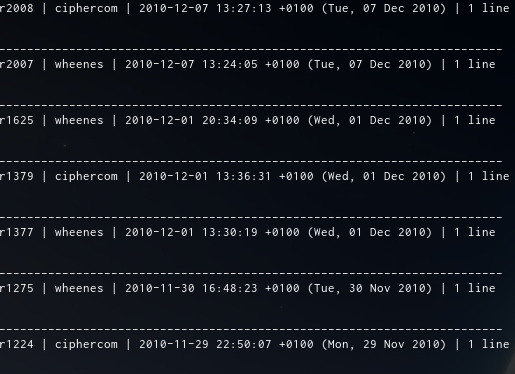
\includegraphics[width=\textwidth]{img/log}
  \end{figure}
\end{frame}
\section{CVCS vs DVCS}
\subsection{CVCS}
\begin{frame}{Aufbau}
  \begin{figure}
    \centering
    \includegraphics[width=\textwidth]{img/cvcs}
  \end{figure}
\end{frame}
\begin{frame}{Workflow}
  \begin{enumerate}[<+->]
  \item Updaten $\rightarrow$ \texttt{svn update}
  \item Änderung machen
  \item Änderungen fixieren $\rightarrow$ \texttt{svn commit}
  \item Änderungen veröffentlichen (Teil von \texttt{svn commit})
  \end{enumerate}
\end{frame}
\subsection{DVCS}
\begin{frame}{Aufbau}
  \begin{figure}
    \centering
    \includegraphics[width=\textwidth]{img/dvcs}
  \end{figure}
\end{frame}
\begin{frame}{Workflow 1 / n}
  \begin{enumerate}[<+->]
  \item Updaten $\rightarrow$ \texttt{git fetch}
  \item Updates mergen $\rightarrow$ \texttt{git merge}
  \item Änderung machen
  \item Änderungen fixieren $\rightarrow$ \texttt{git commit}
  \item Änderungen veröffentlichen $\rightarrow$ \texttt{git push}
  \end{enumerate}
\end{frame}
\begin{frame}{Workflow 2 / n}
  \begin{enumerate}[<+->]
  \item Änderung machen
  \item Änderungen fixieren $\rightarrow$ \texttt{git commit}
  \item GoTo 1
  \item Updaten $\rightarrow$ \texttt{git fetch}
  \item Änderungen auf Updates anpassen $\rightarrow$ \texttt{git rebase}
  \item Änderungen veröffentlichen $\rightarrow$ \texttt{git push}
  \end{enumerate}
\end{frame}
\section{Strategien}
\subsection{Entwicklungsstrategien}

\subsection{Branchstrategien}

\section{Subversion}
\section{Git}
\section{Mercurial}

\section{Anlaufstellen}
\subsection{Handhabung}
\begin{frame}{Git}
  \begin{itemize}[<+->]
  \item \href{http://progit.org/book/}{Progit}
  \item \href{http://www-cs-students.stanford.edu/~blynn/gitmagic/}{Git Magic}
  \item \href{http://www.newartisans.com/2008/04/git-from-the-bottom-up.html}{Git: From Bottom up}
  \item \href{http://www.kernel.org/pub/software/scm/git/docs/gittutorial.html}{Git Tutorial}
  \item \href{http://www.kernel.org/pub/software/scm/git/docs/everyday.html}{Everyday Git}
  \item \href{http://help.github.com/}{Github Bootcamp}
  \end{itemize}
\end{frame}
\begin{frame}{Mercurial}
  \begin{itemize}[<+->]
  \item \href{http://hgbook.red-bean.com/}{Mercurial - The Definitive Guide}
  \item \href{http://hginit.com/}{hg init}
  \item \href{http://mercurial.selenic.com/wiki/Tutorial}{Mercurial Tutorial}
  \item \href{http://mercurial.selenic.com/wiki/UnderstandingMercurial}{Understanding Mercurial}
  \item \href{http://mercurial.selenic.com/guide/}{Learning Mercurial in Workflows}
  \end{itemize}
\end{frame}
\begin{frame}{Subversion}
  \begin{itemize}
  \item \href{http://svnbook.red-bean.com/}{Versionskontrolle mit SVN}
  \end{itemize}
\end{frame}
\subsection{Hosting}
\begin{frame}{Git}
  \begin{itemize}
  \item <1-> \href{http://github.com}{github.com}
    \begin{itemize}
    \item Wiki, Website, Issue Tracker, Teams
    \item Unbegrenzt öffentliche Repositories
    \item Für Studenten: Auf Nachfrage private Repositories
    \end{itemize}
  \item<2-> \href{http://unfuddle.com}{unfuddle.com}
    \begin{itemize}
    \item Issue Tracker
    \item 1 privates Repository
    \end{itemize}
  \item<3-> \href{http://gitorious.org}{gitorious.org}
    \begin{itemize}
    \item Wiki, Issue Tracker, Teams
    \item Unbegrenzt öffentliche Repositories
    \end{itemize}
  \item<4-> ...
  \end{itemize}
\end{frame}
\begin{frame}{Mercurial}
  \begin{itemize}
  \item<1-> \href{http://bitbucket.org}{bitbucket.org}
    \begin{itemize}
    \item Wiki, Website, Issue Tracker, Teams
    \item Unbegrenzt öffentliche Repositories
    \item 5 private Repositories
    \end{itemize}
  \item<2-> ...
  \end{itemize}
\end{frame}
\begin{frame}{Subversion}
  \begin{itemize}
  \item<1-> \href{http://unfuddle.com}{unfuddle.com}
    \begin{itemize}
    \item Issue Tracker
    \item 1 privates Repository
    \end{itemize}
  \item<2-> \href{http://xp-dev.com}{xp-dev.com}
    \begin{itemize}
    \item Wiki, Issue Tracker
    \item 2 private Repositories
    \end{itemize}
  \item<3->
    \href{http://www.rbg.informatik.tu-darmstadt.de/onlinehilfe/freigaben/k\#svn}{Hosting
      bei der RBG}\\(Sollte ähnlich auch für Git und Mercurial funktionieren)
  \item<4-> ...
  \end{itemize}
\end{frame}
\begin{frame}{Alle Drei}
  \begin{itemize}
  \item<1-> \href{http://sourceforge.net}{sourceforge.net}
    \begin{itemize}
    \item Wiki, Website, Issue Tracker
    \end{itemize}
  \item \href{http://code.google.com}{code.google.com}
    \begin{itemize}
    \item Wiki, Website, Issue Tracker
    \end{itemize}
  \item \href{http://assembla.com}{assembla.com}
  \item ...
  \end{itemize}
\end{frame}
\end{document}
